\begin{frame}{Full Restriction ($\PCR[\field]$)}
    
    $\pi \coloneqq (p_1, \dots, p_{\ell})$ is a proof of $\Fs$. $H \coloneqq \{t \mid t \in p_i, \deg(t)
    \text{ is big}\}$.

    \begin{enumerate}
        \item $\pi$ is small $\Rightarrow$ size of $H$ is small.
        \pause
        \item Pick the most frequent literal $x$ in $H$.
        \pause
        \item Set $x$ to $0$ in $\pi$. This operation kills all terms that contain $x$.
        \pause
        \item $\pi \rest (x = 0)$ is still a proof of $\Fs \rest (x = 0)$.
        \pause
        \only<-5>{\item Keep $\Fs \rest (x = 0)$ hard in terms of degree. \begin{tikzpicture}
    \node[inner xsep = 0pt, inner ysep = -20pt, xscale = -1] at (0, 0) {
        
\includegraphics[width = 0.27\textwidth]{pics/cat.png}
    };
    \node at (0pt, -8pt) {};
\end{tikzpicture}
}
        \only<6->{\item Try to avoid local contradictions in $\Fs \rest (x = 0)$. \begin{tikzpicture}
    \node[inner xsep = 0pt, inner ysep = -20pt, xscale = -1] at (0, 0) {
        
\includegraphics[width = 0.27\textwidth]{pics/cat.png}
    };
    \node at (0pt, -8pt) {};
\end{tikzpicture}
}
        \pause
        \pause
            \begin{itemize}
                \item Here we use combinatorial properties of $\Fs$ (expanders graphs, etc.).
            \end{itemize}
        \pause    
        \item Repeat until we have terms of big degree.
    \end{enumerate}

    \vspace{0.3cm}
    \pause
    We kill all terms of big degree but remaining system is still hard in terms of degree.

    \vspace{0.3cm}
    \pause
    \begin{block}{Th (informal). [Razborov 98; Alekhnovich, Razborov 03; Filmus 14]}
        If $\Fs$ is \alert{good} then in low degree we can derive only ``semi-simple'' polynomials, i.e.:
        \begin{itemize}
            \item $p = \sum q_i$;
            \item $q_i \in I_{\text{small subsystem}}$;
            \item leading terms of $q_i$ are different.
        \end{itemize}
    \end{block}
\end{frame}


\begin{frame}{Random $\Delta$-CNF}

    \begin{minipage}{0.3\linewidth}
        \centering
        \onslide<2->{\begin{tikzpicture}

    \pgfmathsetseed{1000007}
    \foreach \i in {0, 1, ..., 5}{
        \node[graph-vert] (b\i) at
            (1.5, 0.4 * \i + 0.4) {};
    }

    \foreach \i in {0, 1, 3, 4, ..., 7}{
        \node[graph-vert = {LEIorange!80!black}{0.15cm}] (a\i) at
            (0, 0.4 * \i) {};

        \foreach \j in {0, 1, 2}{
            \pgfmathsetmacro{\temp}{random(0, 5)}
            \draw (a\i) -- (b\temp);
        }
    }

    \node[graph-vert, fill = green!50] (a2) at (0, 0.8) {};
    \foreach \j in {0, 1, 2}{
        \pgfmathsetmacro{\temp}{random(0, 5)}
        \draw[red, thick] (a2) -- (b\temp);
    }

    \node[below = 0.2cm] at (a0) {$m$};
    \node[below = 0.2cm] at (b0) {$n$};
\end{tikzpicture}}
    \end{minipage}
    \begin{minipage}{0.68\linewidth}
        \begin{enumerate}
            \item Choose $\Delta$ variables uniformly at random: $x_1, \dots, x_{\Delta}$.
            \pause
            \pause
            \item Choose negations uniformly at random: $x_1, \bar{x}_2, \dots, x_{\Delta}$.
            \item Add a constraint: $x_1 \lor \bar{x}_2 \lor \dots \lor x_{\Delta}$
            \item Repeat $m$ times.
        \end{enumerate}
    \end{minipage}

    \pause
    \vspace{0.5cm}
    \begin{itemize}
        \item $m = 6n$ and $\Delta = 3$: whp system is unsatisfiable.
        \item {[Alekhnovich, Razborov 03]} $m = 6n$ and $\Delta \ge 3$: whp any $\PCR[\field]$-refutation
            require $\Omega\left(n\right)$ degree and $2^{\Omega(n)}$ size.
    \end{itemize}
\end{frame}

\begin{frame}{Pigeonhole Principle}

    \begin{minipage}{0.4\linewidth}
        \centering
        \begin{tikzpicture}[>=latex]

    \foreach \i in {1, 2, ..., 6}{
        \node[draw, circle, fill = LEIblue!40, inner sep = 0pt, minimum size = 5pt]
            (a\i) at (0, -0.7 * \i) {};
    }

    \foreach \i in {1, 2, ..., 5}{
        \node[draw, circle, fill = LEIblue!40, inner sep = 0pt, minimum size = 5pt]
            (b\i) at (1.5, -0.7 * \i) {};
    }

    \node[below = 8pt] at (a6) {$m$};
    \node[below = 8pt] at (b5) {$n$};

    
    \draw (a4) -- (b3) node[midway, above] {$x_{i, j}$};
    \draw (a4) -- (b5) node[midway, below] {$x_{i, j'}$};
\end{tikzpicture}
    \end{minipage}
    \pause
    \begin{minipage}{0.58\linewidth}
        \begin{center}
            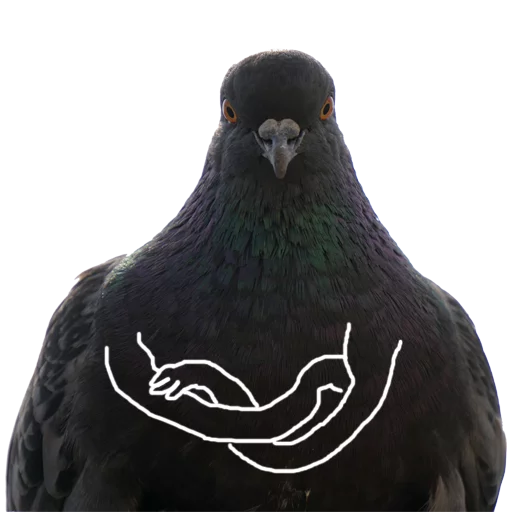
\includegraphics[width = .3\textwidth]{pics/pigeon3.png}
        \end{center}
        \begin{itemize}
            \item $\prod\limits_{j} x_{i, j} = 0$;
            \item $(1 - x_{i, j})(1 - x_{i', j}) = 0$.
        \end{itemize}
    \end{minipage}

    \pause
    \vspace{0.5cm}

    Another distribution, another measure, but the same idea [Razborov' 98; Alekhnovich, Razborov 03].

    \vspace{0.2cm}
    \pause
    \begin{minipage}{0.3\linewidth}
        \centering
        \begin{itemize}
            \item $m = n + 1$ \pause $\color{green!80!black}\checkmark$
        \end{itemize}
    \end{minipage}
    \pause
    \begin{minipage}{0.3\linewidth}
        \centering
        \begin{itemize}
            \item $m \ll n^2$ \pause $\color{green!80!black}\checkmark$
        \end{itemize}
    \end{minipage}
    \pause
    \begin{minipage}{0.3\linewidth}
        \centering
        \begin{itemize}
            \item $m \gg n^2$ \pause \begin{tikzpicture}
    \node[inner xsep = 0pt, inner ysep = -30pt] at (0, 0) {
        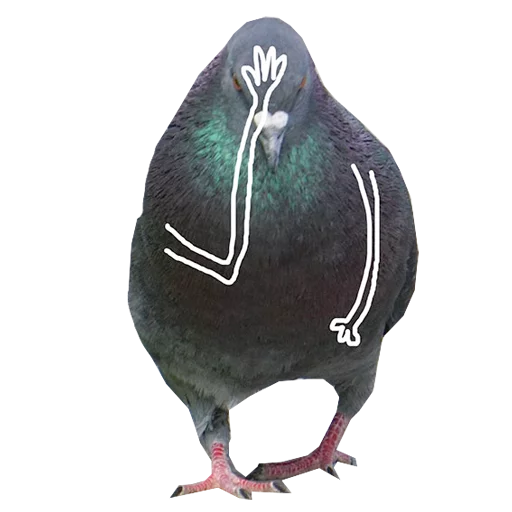
\includegraphics[width = 0.25\textwidth]{pics/pigeon4.png}
    };
    \node at (0pt, -8pt) {};
\end{tikzpicture}

        \end{itemize}
    \end{minipage}
\end{frame}